\documentclass[a4paper,12pt,twoside,final,spanish]{article}
%titlepage: pone el título en una página aparte
%twocolumn
\usepackage{babel} %Para el lenguaje [spanish]
\usepackage[utf8]{inputenc} %Para reconocer todos los símbolos
\usepackage[T1]{fontenc}
\usepackage{textcomp}
\usepackage{amsmath}
\usepackage[makeroom]{cancel} %Para tachar expresiones matemáticas
\usepackage{xcolor}
\newcommand\Ccancel[2][black]{\renewcommand\CancelColor{\color{#1}}\cancel{#2}}
\usepackage{amsfonts}
\usepackage{amssymb}
\usepackage[margin=2cm]{geometry} %Márgenes
\usepackage[T1]{fontenc}
\usepackage[pdftex]{graphicx}
\usepackage{hyperref}
\usepackage{enumerate}
\usepackage{titletoc} %Para hacer el índice
\usepackage{soul} % para tachar texto
\pagestyle{headings}
% Para encerrar expresiones con círculos
\usepackage{mathtools}% superior to amsmath
\usepackage{siunitx} % para escribir grados minutos segundos
\usepackage{tikz}
\makeatletter
\newcommand\mathcircled[1]{%
  \mathpalette\@mathcircled{#1}%
}
\newcommand\@mathcircled[2]{%
  \tikz[baseline=(math.base)] \node[draw,circle,inner sep=1pt] (math) {$\m@th#1#2$};%
}
\makeatother
%---
\usepackage{fancyhdr} %Para usar encabezados y pies personalizados
	\pagestyle{fancy}
	\fancyhf{}
	\fancyhead[LE,RO]{Mecánica del Continuo}
	\fancyhead[RE,LO]{Tensiones Principales}
	\fancyfoot[LE,RO]{Darién Julián Ramírez}
	\fancyfoot[RE,LO]{\thepage}	
	\renewcommand{\footrulewidth}{1pt}
%---
\usepackage{listings} %Para escribir códigos
\lstset{language=XML,
	basicstyle=\footnotesize,
	numbers=left,
 	stepnumber=1,
	numbersep=8pt,
	showspaces=false,               % show spaces adding particular underscores
  	showstringspaces=false,         % underline spaces within strings
  	frame=lines,                   % adds a frame around the code
	tabsize=4,                      
  	captionpos=b,                   % sets the caption-position to bottom
  	breaklines=true,                % sets automatic line breaking
}
%---

\title{\Huge Mecánica del Continuo\\
Trabajo Práctico Nº4\\
Tensiones Principales}
\author{Darién Julián Ramírez}
\date{\vspace{-5ex}}

\begin{document}

\maketitle %Crea la página de título

\section*{Ejercicio 1}

Dado el estado de tensiones de la figura (abajo, izq.), determine: 
\begin{enumerate}[a.]
\item Las tensiones principales 
\item La máxima tensión de corte.  
\end{enumerate}

Ilustre los resultados sobre elementos orientados adecuadamente.

\begin{center}
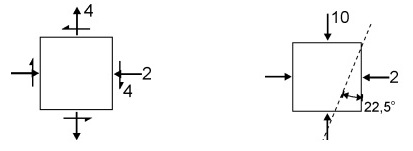
\includegraphics[width=0.7\linewidth,keepaspectratio]{1.jpg}
\end{center}

\dotfill

\[
\sigma=
\left(\begin{matrix}
\sigma_{x} & \tau_{xy} \\
\tau_{yx} & \sigma_{y} \\
\end{matrix}\right)=
\left(\begin{matrix}
-2 & -4 \\
-4 & 4 \\
\end{matrix}\right)
\]

\[
\textit{Para Mohr:}\quad A=(-2,4);\quad B=(4,-4)
\]

\begin{center}
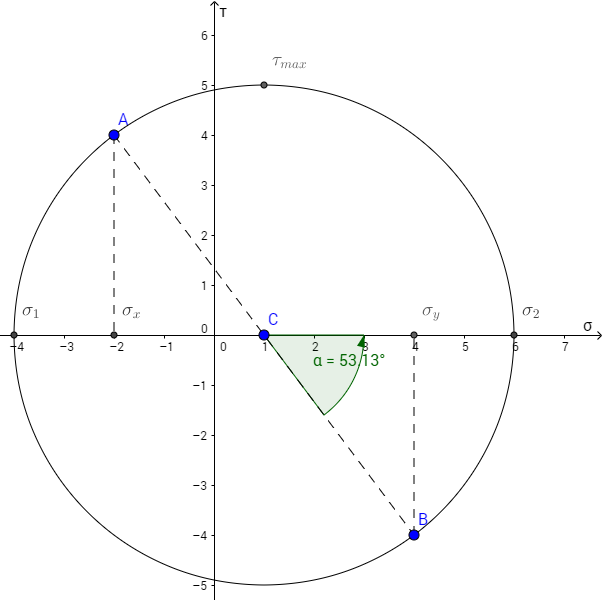
\includegraphics[width=0.9\linewidth,keepaspectratio]{mohr_ej1.png}
\end{center}

Tensiones principales:

\[
(\sigma_{1},\sigma_{2})=\frac{\sigma_{x}+\sigma_{y}}{2}\pm\sqrt{\left(\frac{\sigma_{x}-\sigma_{y}}{2}\right)^{2}+\tau_{xy}^{2}}
=
\frac{-2+4}{2}\pm\sqrt{\left(\frac{-2-4}{2}\right)^{2}+(-4)^{2}}
\]
\[
=1\pm 5=(-4,6)\implies
\left(\begin{matrix}
-4 & 0 \\
0 & 6 \\
\end{matrix}\right)
\]

\textit{El $\sigma_{1}$ se corresponde con el punto $A$. El $\sigma_{2}$ se corresponde con el punto $B$.}\\

Corte máximo:

\[
\tau_{max}=\frac{\sigma_{max}-\sigma_{min}}{2}=\frac{6-(-4)}{2}=5
\]

O también:

\[
\tau_{max}=\sqrt{\left(\frac{\sigma_{x}-\sigma_{y}}{2}\right)^{2}+\tau_{xy}^{2}}
=\sqrt{\left(\frac{-2-4}{2}\right)^{2}+(-4)^{2}}=5
\]

Extra: \textit{$\theta$ es el ángulo para el cual las tensiones de corte se hacen cero y solo quedan las tensiones principales.}

\[
\alpha=2\theta;\quad
\tan{2\theta}=\frac{2\tau_{xy}}{\sigma_{x}-\sigma_{y}}
\implies
\theta=\frac{\tan^{-1}\left(\frac{2\tau_{xy}}{\sigma_{x}-\sigma_{y}}\right)}{2}
=\frac{\tan^{-1}\left(\frac{2(-4)}{-2-4}\right)}{2}=\ang{26;33;54.18}
\]

\section*{Ejercicio 2}

Las tensiones dadas en la figura (arriba, der.) son tensiones principales. Determine las tensiones que actúan en un plano orientado a un ángulo de 22,5 grados con el eje 
vertical, como se muestra.

\dotfill  

\[
\sigma=
\left(\begin{matrix}
\sigma_{1} & 0 \\
0 & \sigma_{2} \\
\end{matrix}\right)=
\left(\begin{matrix}
-2 & 0 \\
0 & -10 \\
\end{matrix}\right);\quad\theta=-\ang{22.5}
\]

\[
\textit{Para Mohr:}\quad A=(-2,0);\quad B=(-10,0);\quad\alpha
=2\theta=2\cdot (-\ang{22.5})=-\ang{45}
\]

\begin{center}
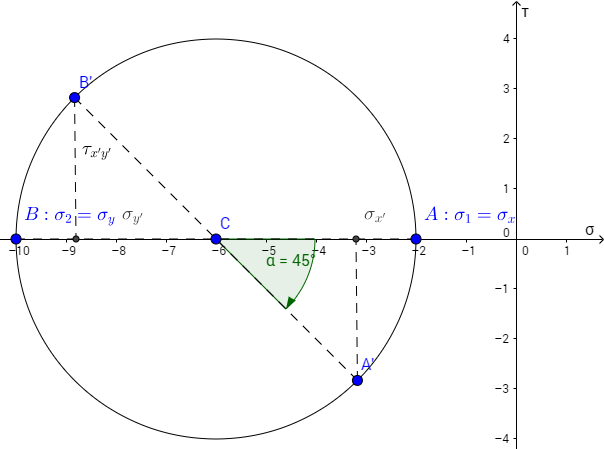
\includegraphics[width=0.9\linewidth,keepaspectratio]{mohr_ej2.png}
\end{center}

\[
\sigma_{x'}=\frac{\sigma_{x}+\sigma_{y}}{2}+\frac{\sigma_{x}-\sigma_{y}}{2}\cos{2\theta}+\tau_{xy}\sin{2\theta}
\]
\[
=\frac{-2+(-10)}{2}+\frac{-2+10}{2}\cos{\ang{-45}}+0\cdot\sin{\ang{-45}}
=-6+2\sqrt{2}+0=-3.171572875
\]
\\
\[
\sigma_{y'}=\frac{\sigma_{x}+\sigma_{y}}{2}-\frac{\sigma_{x}-\sigma_{y}}{2}\cos{2\theta}-\tau_{xy}\sin{2\theta}
\]
\[
=\frac{-2+(-10)}{2}-\frac{-2+10}{2}\cos{\ang{-45}}-0\cdot\sin{\ang{-45}}
=-6-2\sqrt{2}-0=-8.828427125
\]

\[
\tau_{x'y'}=-\frac{\sigma_{x}-\sigma_{y}}{2}\sin{2\theta}+\tau_{xy}\cos{2\theta}
\]
\[
=-\frac{-2+10}{2}\sin{-\ang{45}}+0\cdot\cos{-\ang{45}}=2\sqrt{2}=2.828427125
\]

\[
\sigma=
\left(\begin{matrix}
\sigma_{x} & \tau_{xy} \\
\tau_{yx} & \sigma_{y} \\
\end{matrix}\right)=
\left(\begin{matrix}
-3.171572875 & 2.828427125 \\
2.828427125 & -8.828427125 \\
\end{matrix}\right)
\]\\

Verificación del invariante:

\[
\sigma_{x'}+\sigma_{y'}=-3.171572875-8.828427125=-12=-2-10=\sigma_{x}+\sigma_{y}
\]

\section*{Ejercicio 3}

George Stokes dio en 1850 la solución al problema de una esfera moviéndose en un 
fluido viscoso (Newtoniano) a velocidad constante $U$. Sobre la superficie de la esfera, las tres componentes del vector de tensiones son:

\[
\stackrel r T_{x}=-\frac{x}{a}p_{0}+\frac{3}{2}\mu\frac{U}{a};\quad
\stackrel r T_{y}=-\frac{y}{a}p_{0};\quad
\stackrel r T_{z}=-\frac{z}{a}p_{0}
\]

\begin{center}
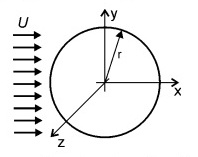
\includegraphics[width=0.3\linewidth,keepaspectratio]{2.jpg}
\end{center}

¿Cuál es la fuerza resultante que actúa sobre la esfera?

\dotfill

\[
dF=\mathbf{T}ds;\quad R=\int_{s}dF=\int_{s}T.ds
\]

\[
R_{x}=\int T_{x}dS;\quad R_{y}\int T_{y}dS=\phi
\]

\[
R_{x}=\int_{s}T_{x}dS=\int_{s}-\frac{x}{a}p_{0}dS+\int_{s}\frac{3}{2}\mu\frac{U}{a}dS
=\frac{3}{2}\mu\frac{U}{a}\int_{s}dS=6\pi\mu aU
\]

\[
R=
\left(\begin{matrix}
6\pi aU \\
0 \\
0 \\
\end{matrix}\right)
\]

\section*{Ejercicio 4}

Sean $\tau_{xx}=1000$, $\tau_{yy}=-1000$, $\tau_{zz}=0$, $\tau_{xy}=500$, $\tau_{yz}=-200$, $\tau_{zx}=0$. ¿Cuánto vale la tracción total que actúa sobre una superficie cuyo versor normal es: $\mathbf{v}=0.1\mathbf{i}+0.3\mathbf{j}+\sqrt{0.9}\mathbf{k}$?

¿Cuáles son las tres componentes (en las direcciones $x,y,z$) del vector de tensión
actuando sobre esta superficie? ¿Cuál es la tensión normal actuando sobre esta superficie? ¿Cuál es la tensión de corte resultante que actúa sobre la superficie?

\dotfill

Tensor de tensiones y versor normal a la superficie:

\[
\tau=\left(\begin{matrix}
\tau_{xx} & \tau_{xy} & \tau_{xz} \\
\tau_{yx} & \tau_{yy} & \tau_{yz} \\
\tau_{zx} & \tau_{zy} & \tau_{zz} \\
\end{matrix}\right)=
\left(\begin{matrix}
1000 & 500 & 0 \\
500 & -1000 & -200 \\
0 & -200 & 0 \\
\end{matrix}\right);\quad
\nu=\left(\begin{matrix}
0.1 \\
0.3 \\
\sqrt{0.9} \\
\end{matrix}\right)
\]\\

Vector de tensión:

\[
\stackrel \nu T_{i}=\sigma_{ij}\nu_{j}=
\left(\begin{matrix}
1000 & 500 & 0 \\
500 & -1000 & -200 \\
0 & -200 & 0 \\
\end{matrix}\right)\cdot
\left(\begin{matrix}
0.1 \\
0.3 \\
\sqrt{0.9} \\
\end{matrix}\right)=
\left(\begin{matrix}
250 \\
-439.737 \\
-60 \\
\end{matrix}\right)
\]\\

Componentes del vector de tensión:

\[
\stackrel \nu T_{x}=250;\quad
\stackrel \nu T_{y}=-439.737\approx-440;\quad
\stackrel \nu T_{z}=-60;
\]\\

Componente normal del vector de tensión:

\[
T^{(n)}=(\stackrel \nu T\cdot\nu)\nu=
\left(\left(\begin{matrix}
250 \\
-439.737 \\
-60 \\
\end{matrix}\right)\cdot
\left(\begin{matrix}
0.1 \\
0.3 \\
\sqrt{0.9} \\
\end{matrix}\right)\right)
\left(\begin{matrix}
0.1 \\
0.3 \\
\sqrt{0.9} \\
\end{matrix}\right)=
\left(\begin{matrix}
-16.384 \\
-49.153 \\
-155.434 \\
\end{matrix}\right)
\]\\

Componente tangencial del vector de tensión:

\[
T^{(c)}=\stackrel \nu T-T^{(n)}=
\left(\begin{matrix}
250 \\
-439.737 \\
-60 \\
\end{matrix}\right)-
\left(\begin{matrix}
-16.384 \\
-49.153 \\
-155.434 \\
\end{matrix}\right)=
\left(\begin{matrix}
266.384 \\
-390.584 \\
95.434 \\
\end{matrix}\right)
\]\\

\section*{Ejercicio 5}

Si el estado de tensiones en un punto $(x_{0},y_{0},z_{0})$ es:

\[
\sigma_{ij}=
\left(\begin{matrix}
1 & 0 & -1\\
0 & -1 & 0\\
-1 & 0 & 1\\
\end{matrix}\right)
\]

Hallar los valores de los invariantes $I_{1},I_{2},I_{3}$ y las tensiones principales.

\dotfill

\[
|\sigma_{ij}-\sigma\delta_{ij}|=
\left|\begin{matrix}
1-\sigma & 0 & -1 \\
0 & -1-\sigma & 0 \\
-1 & 0 & 1-\sigma \\
\end{matrix}\right|=0
\]

\[
\implies -\sigma^{3}+I_{1}\sigma^{2}-I_{2}\sigma+I_{3}=0
\]

Cálculo de invariantes:

\[
I_{1}=\tau_{11}+\tau_{22}+\tau_{33}
=1-1+1=1
\]\\

\[
I_{2}=
\left|\begin{matrix}
\tau_{22} & \tau_{23} \\
\tau_{32} & \tau_{33} \\
\end{matrix}\right|
+
\left|\begin{matrix}
\tau_{11} & \tau_{13} \\
\tau_{31} & \tau_{33} \\
\end{matrix}\right|
+
\left|\begin{matrix}
\tau_{11} & \tau_{12} \\
\tau_{21} & \tau_{22} \\
\end{matrix}\right|
=
\left|\begin{matrix}
-1 & 0 \\
0 & 1 \\
\end{matrix}\right|
+
\left|\begin{matrix}
1 & -1 \\
-1 & 1 \\
\end{matrix}\right|
+
\left|\begin{matrix}
1 & 0 \\
0 & -1 \\
\end{matrix}\right|
\]
\[
=-1+(1-1)+(-1)=-1+0+(-1)=-2
\]\\

\[
I_{3}=
\left|
\begin{matrix}
\tau_{11} & \tau_{12} & \tau_{13} \\
\tau_{21} & \tau_{22} & \tau_{23} \\
\tau_{31} & \tau_{32} & \tau_{33} \\
\end{matrix}
\right|
=
\tau_{11}
\left|\begin{matrix}
\tau_{22} & \tau_{23} \\
\tau_{32} & \tau_{33} \\
\end{matrix}\right|
-
\tau_{12}
\left|\begin{matrix}
\tau_{21} & \tau_{23} \\
\tau_{31} & \tau_{33} \\
\end{matrix}\right|
+
\tau_{13}
\left|\begin{matrix}
\tau_{21} & \tau_{22} \\
\tau_{31} & \tau_{32} \\
\end{matrix}\right|
\]
\[
=
1\cdot
\left|\begin{matrix}
-1 & 0 \\
0 & 1 \\
\end{matrix}\right|
-
\left(
0\cdot
\left|\begin{matrix}
0 & 0 \\
-1 & 1 \\
\end{matrix}\right|\right)
+
-1\cdot
\left|\begin{matrix}
0 & -1 \\
-1 & 0 \\
\end{matrix}\right|
=-1+0+1=0
\]\\

Cálculo de las tensiones principales:

\[
\implies -\sigma^{3}+\sigma^{2}+2\sigma=0
\implies \sigma(-\sigma^{2}+\sigma+2)=0 \implies \sigma_{1}=0
\]

\[
-\sigma^{2}+\sigma+2=0
\implies \frac{-1\pm\sqrt{1^{2}-4\cdot (-1)\cdot 2}}{2\cdot(-1)}
=\frac{-1\pm 3}{-2}
\]
\[
\implies \sigma_{2}=-1;\quad \sigma_{3}=2
\]\\

Cálculo de las direcciones principales:

\[
(\sigma_{ij}-\sigma\delta_{ij})\cdot\nu_{j}=0
\]

Para $\sigma_{1}=0$:

\[
\sigma_{ij}\cdot\nu_{j}=
\left(\begin{matrix}
1 & 0 & -1 \\
0 & -1 & 0 \\
-1 & 0 & 1 \\
\end{matrix}\right)\cdot
\left(\begin{matrix}
\stackrel \sigma \nu_{1} \\
\stackrel \sigma \nu_{2} \\
\stackrel \sigma \nu_{3} \\
\end{matrix}\right)
=
\left(\begin{matrix}
\stackrel \sigma \nu_{1}-\stackrel \sigma \nu_{3} \\
\stackrel \sigma \nu_{2} \\
-\stackrel \sigma \nu_{1}+\stackrel \sigma \nu_{3} \\
\end{matrix}\right)
=
\left(\begin{matrix}
0 \\
0 \\
0 \\
\end{matrix}\right)
\]

\[
\stackrel \sigma \nu_{1}-\stackrel \sigma \nu_{3}=0
\implies \stackrel \sigma \nu_{1}=\stackrel \sigma \nu_{3}
\]
\[
\stackrel \sigma \nu_{2}=0
\]
\[
-\stackrel \sigma \nu_{1}+\stackrel \sigma \nu_{3}=0
\implies \stackrel \sigma \nu_{3}=\stackrel \sigma \nu_{1}
\]
\[
\implies
\mathbf{v}=\left(\begin{matrix}
\alpha \\
0 \\
\alpha \\
\end{matrix}\right);\quad
\|\mathbf{v}\|
=\sqrt{\alpha^2+0^2+\alpha^2}=\sqrt{2\alpha^2}=\sqrt{2}\alpha
\]

\[
\nu_{\sigma_{1}}=\frac{\mathbf{v}}{\|\mathbf{v}\|}
=
\left(\frac{1}{\sqrt{2}},0,\frac{1}{\sqrt{2}}\right)^{T}
\]

Para $\sigma_{2}=-1$:

\[
(\sigma_{ij}-\sigma_{2}\delta_{ij})\cdot\nu_{j}=
\left(\begin{matrix}
2 & 0 & -1 \\
0 & 0 & 0 \\
-1 & 0 & 2 \\
\end{matrix}\right)\cdot
\left(\begin{matrix}
\stackrel \sigma \nu_{1} \\
\stackrel \sigma \nu_{2} \\
\stackrel \sigma \nu_{3} \\
\end{matrix}\right)
=
\left(\begin{matrix}
2\stackrel \sigma \nu_{1}-\stackrel \sigma \nu_{3} \\
0 \\
-\stackrel \sigma \nu_{1}+2\stackrel \sigma \nu_{3} \\
\end{matrix}\right)
=
\left(\begin{matrix}
0 \\
0 \\
0 \\
\end{matrix}\right)
\]

\[
2\stackrel \sigma \nu_{1}-\stackrel \sigma \nu_{3}=0
\implies 2\stackrel \sigma \nu_{1}=\stackrel \sigma \nu_{3}
\]
\[
\implies 2\cdot2\stackrel \sigma \nu_{3}=\stackrel \sigma \nu_{3}
\implies 4\stackrel \sigma \nu_{3}=\stackrel \sigma \nu_{3}
\implies 4\stackrel \sigma \nu_{3}-\stackrel \sigma \nu_{3}=0
\implies 3\stackrel \sigma \nu_{3}=0
\implies \stackrel \sigma \nu_{3}=0
\]
\[
0=0
\]
\[
-\stackrel \sigma \nu_{1}+2\stackrel \sigma \nu_{3}=0
\implies 2\stackrel \sigma \nu_{3}=\stackrel \sigma \nu_{1}
\]
\[
\stackrel \sigma \nu_{1}=0
\]

\[
\implies
\mathbf{v}=\left(\begin{matrix}
0 \\
\alpha \\
0 \\
\end{matrix}\right);\quad
\|\mathbf{v}\|
=\sqrt{0^2+\alpha^2+0^2}=\sqrt{\alpha^2}=\alpha
\]

\[
\nu_{\sigma_{2}}=\frac{\mathbf{v}}{\|\mathbf{v}\|}
=
\left(0,1,0\right)^{T}
\]

Para $\sigma_{3}=2$:

\[
(\sigma_{ij}-\sigma_{3}\delta_{ij})\cdot\nu_{j}=
\left(\begin{matrix}
-1 & 0 & -1 \\
0 & -3 & 0 \\
-1 & 0 & -1 \\
\end{matrix}\right)\cdot
\left(\begin{matrix}
\stackrel \sigma \nu_{1} \\
\stackrel \sigma \nu_{2} \\
\stackrel \sigma \nu_{3} \\
\end{matrix}\right)
=
\left(\begin{matrix}
-\stackrel \sigma \nu_{1}-\stackrel \sigma \nu_{3} \\
-3\stackrel \sigma \nu_{2} \\
-\stackrel \sigma \nu_{1}-\stackrel \sigma \nu_{3} \\
\end{matrix}\right)
=
\left(\begin{matrix}
0 \\
0 \\
0 \\
\end{matrix}\right)
\]

\[
-\stackrel \sigma \nu_{1}-\stackrel \sigma \nu_{3}=0
\implies \stackrel \sigma \nu_{1}=-\stackrel \sigma \nu_{3}
\]
\[
-3\stackrel \sigma \nu_{2}=0
\implies \stackrel \sigma \nu_{2}=0
\]
\[
-\stackrel \sigma \nu_{1}-\stackrel \sigma \nu_{3}=0
\implies \stackrel \sigma \nu_{3}=-\stackrel \sigma \nu_{1}
\]

\[
\implies
\mathbf{v}=\left(\begin{matrix}
\alpha \\
0 \\
-\alpha \\
\end{matrix}\right);\quad
\|\mathbf{v}\|
=\sqrt{\alpha^2+0^2+(-\alpha)^2}=\sqrt{\alpha^2+\alpha^2}=\sqrt{2\alpha^2}=\sqrt{2}\alpha
\]

\[
\nu_{\sigma_{3}}=\frac{\mathbf{v}}{\|\mathbf{v}\|}
=
\left(\frac{1}{\sqrt{2}},0,-\frac{1}{\sqrt{2}}\right)^{T}
\]

Matriz de rotación:

\[
\beta=
\left(\begin{matrix}
\nu_{\sigma_{2}}^{T} \\
\nu_{\sigma_{1}}^{T} \\
\nu_{\sigma_{3}}^{T} \\
\end{matrix}\right)
=
\left(\begin{matrix}
0 & 1 & 0 \\
\frac{1}{\sqrt{2}} & 0 & \frac{1}{\sqrt{2}} \\
\frac{1}{\sqrt{2}} & 0 & -\frac{1}{\sqrt{2}} \\
\end{matrix}\right);\quad
|\beta|=1>0
\]

\section*{Ejercicio 6}

Sea $\tau_{ij}$ un tensor de tensiones. Evaluar los productos:

\begin{enumerate}[a.]
\item $\varepsilon_{ijk}\tau_{jk}$

\begin{quote}
$\varepsilon_{ijk}\tau_{jk}
\hfill\textit{Sólo quedan los épsilon distintos de cero.}\\
=\varepsilon_{123}\tau_{23}+\varepsilon_{231}\tau_{31}+\varepsilon_{312}\tau_{12}+
\varepsilon_{321}\tau_{21}+\varepsilon_{213}\tau_{13}+\varepsilon_{132}\tau_{32}
\hfill\textit{Definición de $\varepsilon$.}\\
=\tau_{23}+\tau_{31}+\tau_{12}-\tau_{21}-\tau_{13}-\tau_{32}
\hfill\textit{Por simetría de $\tau$.}\\
=\Ccancel[blue]{\tau_{23}}
\Ccancel[red]{+\tau_{31}}
\Ccancel[green]{+\tau_{12}}
\Ccancel[green]{-\tau_{12}}
\Ccancel[red]{-\tau_{31}}
\Ccancel[blue]{-\tau_{23}}
=0$\\

Otra forma de demostrarlo:

$\varepsilon_{ijk}\tau_{jk}
\hfill\textit{Rotación no cíclica de épsilon.}\\
=-\varepsilon_{ikj}\tau_{jk}
\hfill\textit{Por simetría de $\tau$.}\\
=-\varepsilon_{ikj}\tau_{kj}
\hfill\textit{Sea k=m.}\\
=-\varepsilon_{imj}\tau_{mj}
\hfill\textit{Sea j=k.}\\
=-\varepsilon_{imk}\tau_{mk}
\hfill\textit{Sea m=j.}\\
=-\varepsilon_{ijk}\tau_{jk}\\
\implies \varepsilon_{ijk}\tau_{jk}=-\varepsilon_{ijk}\tau_{jk}\\
\implies \varepsilon_{ijk}\tau_{jk}+\varepsilon_{ijk}\tau_{jk}=0\\
\implies 2\varepsilon_{ijk}\tau_{jk}=0\\
\implies \varepsilon_{ijk}\tau_{jk}=0$
\end{quote}

\item $\varepsilon_{ijk}\varepsilon_{ist}\tau_{kt}$

\begin{quote}
$\varepsilon_{ijk}\varepsilon_{ist}\tau_{kt}
\hfill\textit{Identidad épsilon-delta.}\\
=(\delta_{js}\delta_{kt}-\delta_{jt}\delta_{ks})\tau_{kt}
\hfill\textit{Distribuyendo.}\\
=\delta_{js}\delta_{kt}\tau_{kt}-\delta_{jt}\delta_{ks}\tau_{kt}
\hfill\textit{Contrayendo índices.}\\
=\delta_{js}\tau_{tt}-\tau_{sj}
\hfill \sigma_{0}=\frac{\sigma_{kk}}{3} \implies \sigma_{kk}=3\sigma_{0};\quad
\tau_{sj}=\tau_{js}\\
=3\delta_{js}\sigma_{0}-\tau_{js}$
\end{quote}
\end{enumerate}

\section*{Ejercicio 7}

Dibuje el círculo de Mohr para:

\begin{enumerate}[a.]
\item Tensión uniaxial pura.

\begin{quote}
\[
\sigma=
\left(\begin{matrix}
\sigma_{x} & 0 \\
0 & 0 \\
\end{matrix}\right)
\]

\begin{center}
\begin{tabular}{c c}
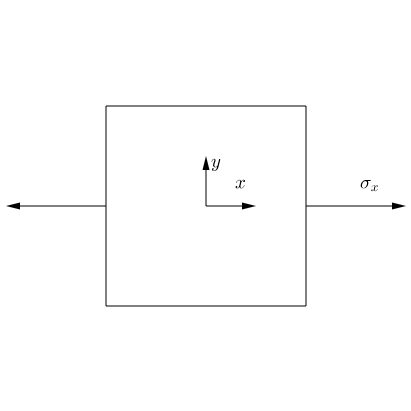
\includegraphics[width=0.5\linewidth,keepaspectratio]{cu_tup.png} &
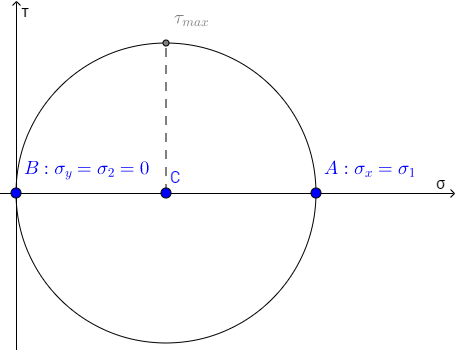
\includegraphics[width=0.5\linewidth,keepaspectratio]{mohr_tup.png}
\end{tabular}
\end{center}
\end{quote}

\item Compresión uniaxial pura.

\begin{quote}
\[
\sigma=
\left(\begin{matrix}
-\sigma_{x} & 0 \\
0 & 0 \\
\end{matrix}\right)
\]

\begin{center}
\begin{tabular}{c c}
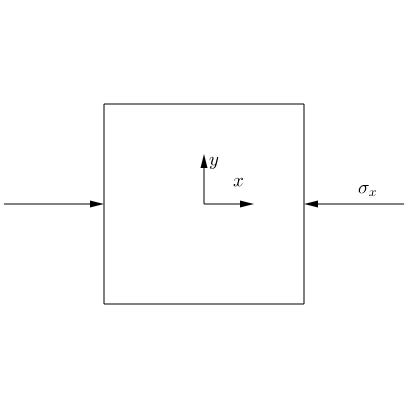
\includegraphics[width=0.5\linewidth,keepaspectratio]{cu_cup.png} &
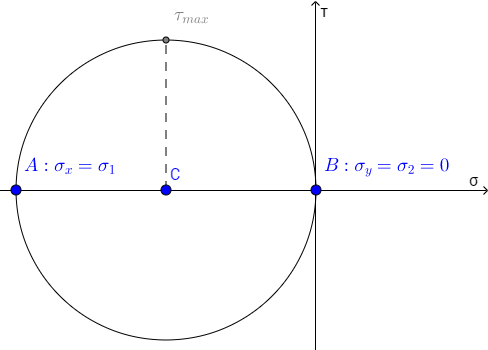
\includegraphics[width=0.5\linewidth,keepaspectratio]{mohr_cup.png}
\end{tabular}
\end{center}
\end{quote}

\item Tensión biaxial pura.

\begin{quote}
\[
\sigma=
\left(\begin{matrix}
\sigma_{x} & 0 \\
0 & \sigma_{y} \\
\end{matrix}\right);\quad \sigma_{x}>\sigma_{y}
\]

\begin{center}
\begin{tabular}{c c}
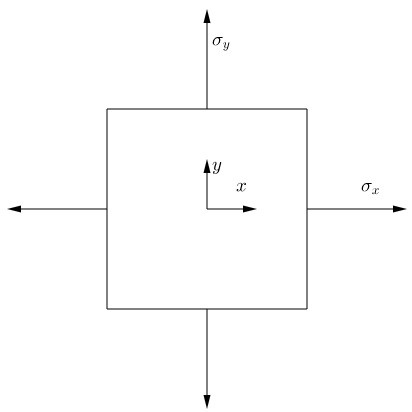
\includegraphics[width=0.5\linewidth,keepaspectratio]{cu_tbp.png} &
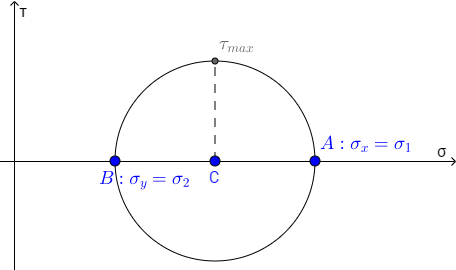
\includegraphics[width=0.5\linewidth,keepaspectratio]{mohr_tbp.png}
\end{tabular}
\end{center}
\end{quote}

\item Corte puro.

\begin{quote}
\[
\sigma=
\left(\begin{matrix}
0 & \tau_{xy} \\
\tau_{yx} & 0 \\
\end{matrix}\right)
\]

\begin{center}
\begin{tabular}{c c}
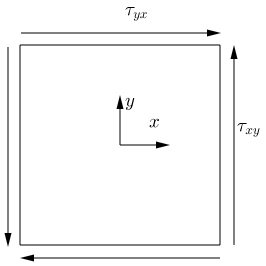
\includegraphics[width=0.5\linewidth,keepaspectratio]{cu_cp.png} &
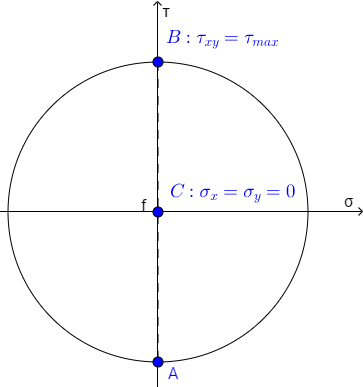
\includegraphics[width=0.5\linewidth,keepaspectratio]{mohr_cp.png}
\end{tabular}
\end{center}
\end{quote}

\end{enumerate}

\section*{Ejercicio 8}

\textit{Concentración de tensiones.} Describa las condiciones de borde para una placa con un agujero circular sometida a una carga de tracción estática uniforme con tensión normal $\sigma_{x}=cte=p$ actuando en los extremos.
 
Si esta placa está hecha con un material elástico lineal, se sabe que la solución es: 

\[
\sigma_{r}=\frac{p}{2}\left(1-\frac{a^{2}}{r^{2}}\right)\left[1+\left(1-3\frac{a^{2}}{r^{2}}\right)\cos{2\theta}\right]
\]

\[
\sigma_{\theta}=\frac{p}{2}\left[1+\frac{a^{2}}{r^{2}}-\left(1+3\frac{a^{4}}{r^{4}}\right)\cos{2\theta}\right]
\]

\[
\tau_{r\theta}=-\frac{p}{2}\left(1-\frac{a^2}{r^2}\right)\left(1+3\frac{a^2}{r^2}\right)\sin{2\theta}
\]

\begin{center}
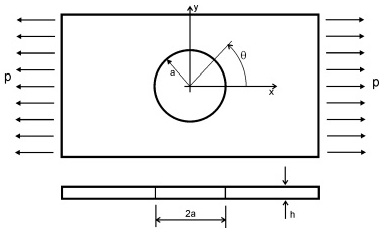
\includegraphics[width=0.5\linewidth,keepaspectratio]{3.jpg}
\end{center}

\begin{enumerate}[a.]
\item Verifique las condiciones de borde para ver si éstas se satisfacen.
\item Encuentre la ubicación del punto donde la tensión normal $\sigma_{theta}$ es máxima.
\item Encuentre la máxima tensión de corte en toda la placa.
\item Obtenga la máxima tensión principal en toda la placa.
\item Realice la visualización de campos de tensión utilizando software como Matlab u Octave. Ver la distribución obtenida y valores obtenidos. Identificar los puntos donde se hacen máximos cada una de las componentes de tensión.
\item \textit{(Opcional)} Asigne valores a las dimensiones de la placa. Calcule la solución usando un software de elementos finitos. Compare la solución obtenida con la solución analítica obtenida en el punto anterior.
\end{enumerate}

Nota: verá que la tensión es máxima en torno al agujero. Este fenómeno es llamado 
concentración de tensiones.

\dotfill

Las coordenadas están dadas en la forma polar suponiendo:

\[
\begin{array}{ccc}
r\to\infty; &
\theta\to 0; &
\sigma\nu
=\begin{pmatrix}
\sigma_{r}      & \tau_{r\theta} \\
\tau_{\theta r} & \sigma_{\theta}
\end{pmatrix}
\cdot
\begin{pmatrix}
1 \\
0
\end{pmatrix}
=\begin{pmatrix}
\sigma_{r} \\
\tau_{r\theta}
\end{pmatrix}
=\begin{pmatrix}
p \\
0
\end{pmatrix};
\mbox{ En el borde superior.}
\end{array}
\] 

En $\theta$:

\[
\frac{\partial\sigma_{0}}{\partial\theta}
=p\left(1+\frac{3a^{4}}{r^{4}}\right)\sin 2\theta=0;
\text{ Es cero cuando el seno es cero.}
\]

En $r$:

\[
\frac{\partial\sigma_{0}}{\partial r}
=-p\frac{a^{2}}{r^{3}}+\frac{6a^{4}p\cos 2\theta}{r^{5}}=0
\]

\[
-pa^{2}+\frac{6pa^{4}\cos{n\theta}}{r^{2}}=0
\]

\[
pa^{2}=6\frac{pa^{4}}{r^{2}}(-1)^{n}
\implies
r=\sqrt{6a^{2}(-1)^{n}}
\left\{
\begin{array}{l}
\text{Si $n$ es impar $\implies r\in\mathbb{R}$.} \\
\text{Si $n$ es par $\implies r=\sqrt{6}a$.}
\end{array}
\right.
\]

También se evalúa en los extremos: 
$r=\sqrt{6}a;\quad
\theta=n\pi \implies \theta_{0}=\frac{p}{24}$

\[
r\to\infty;  \quad
\theta=n\pi; \quad
r_{\theta}=\frac{p}{2}(1-\cos{2n\pi})=0
\]

\[
\begin{array}{llcl}
r=a        & \theta=n\pi          & \implies & \sigma_{0}=-p \\
r=a        & \theta=\frac{\pi}{2} & \implies & \sigma_{0}=3p \\
r\to\infty & \theta=\frac{\pi}{2} & \implies & \sigma_{0}=p
\end{array}
\]

Los máximos se van a dar en el borde del agujero.

\section*{Apéndice}

Dado el tensor de tensiones:

\[
\sigma_{ij}=
\left(\begin{matrix}
\sigma_{x} & \tau_{xy} & \tau_{xz}\\
\tau_{yx} & \sigma_{y} & \tau_{yz}\\
\tau_{zx} & \tau_{zy} & \sigma_{z}\\
\end{matrix}\right)
\]

Las tensiones principales son los elementos de la diagonal del nuevo tensor de tensiones que resulta de rotar el tensor anterior haciendo a las tensiones de cortes nulas:

\[
\sigma_{ij}=
\left(\begin{matrix}
\sigma_{x} & 0 & 0\\
0 & \sigma_{y} & 0\\
0 & 0 & \sigma_{z}\\
\end{matrix}\right)
\]

\subsection*{Estado Plano de Tensiones}

No hay tensiones en la dirección de $z$:

\[
\sigma_{ij}'=\beta_{ik}\sigma_{kj}=
\left(\begin{matrix}
\cos\theta & \sin\theta & 0\\
-\sin\theta & \cos\theta & 0\\
0 & 0 & 1\\
\end{matrix}\right)
\left(\begin{matrix}
\sigma_{x} & \tau_{xy} & 0\\
\tau_{yx} & \sigma_{y} & 0\\
0 & 0 & 0\\
\end{matrix}\right)=
\left(\begin{matrix}
\sigma_{x'} & \tau_{x'y'} & 0\\
\tau_{y'x'} & \sigma_{y'} & 0\\
0 & 0 & 0\\
\end{matrix}\right)
\]
\\
\[
\sigma_{x'}=\frac{\sigma_{x}+\sigma_{y}}{2}+\frac{\sigma_{x}-\sigma_{y}}{2}\cos{2\theta}+\tau_{xy}\sin{2\theta}
\]

\[
\sigma_{y'}=\frac{\sigma_{x}+\sigma_{y}}{2}-\frac{\sigma_{x}-\sigma_{y}}{2}\cos{2\theta}-\tau_{xy}\sin{2\theta}
\]

\[
\tau_{x'y'}=-\frac{\sigma_{x}-\sigma_{y}}{2}\sin{2\theta}+\tau_{xy}\cos{2\theta}
\]

\[
\textit{Invariante: }\sigma_{x'}+\sigma_{y'}=\sigma_{x}+\sigma_{y}
\]

\[
\frac{\partial\sigma_{x'}}{\partial\theta}=2\tau_{x'y'};\quad\frac{\partial\sigma_{y'}}{\partial\theta}=-2\tau_{xy}
\]

\[
\textit{Cuando }\tau_{x'y'}=0\implies\tan{2\theta}=\frac{2\tau_{xy}}{\sigma_{x}-\sigma_{y}}
\]

\[
\textit{Tensiones principales: }(\sigma_{1},\sigma_{2})=\frac{\sigma_{x}+\sigma_{y}}{2}\pm\sqrt{\left(\frac{\sigma_{x}-\sigma_{y}}{2}\right)^{2}+\tau_{xy}^{2}}
\]

\[
\textit{Corte máximo: }\tau_{max}=\frac{\sigma_{max}-\sigma_{min}}{2}=\sqrt{\left(\frac{\sigma_{x}-\sigma_{y}}{2}\right)^{2}+\tau_{xy}^{2}}
\]

\subsection*{Círculo de Mohr}

Será planteado para el siguiente ejemplo:\\

\begin{center}
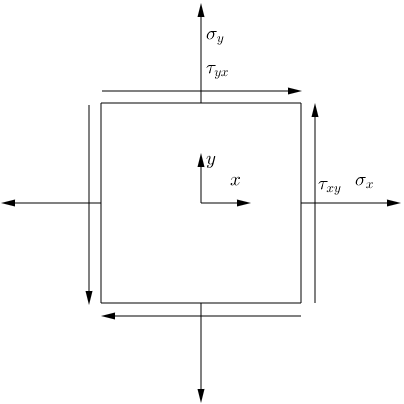
\includegraphics[width=0.5\linewidth,keepaspectratio]{cu.png}
\end{center}

Se procede a armar el tensor de tensiones. Como se puede observar tanto $\sigma_{x}$ como $\sigma_{y}$ están traccionando la chapa, es decir, son positivas.

Para determinar el signo de $\tau_{xy}$ se debe observar el sentido en el que produce el corte. Recuérdese que los subíndices significan: \textbf{cara sobre la que actúa la tensión} y \textbf{sentido sobre el que actúa la tensión} ($\tau_{cara,sentido}$). Entonces, si el sentido de corte es el mismo al de la cara sobre el que actúa, $\tau_{xy}$ será positivo, en caso contrario será negativo. Finalmente $\tau_{yx}=\tau_{xy}$ por simetría del tensor de tensiones.\\

Para este ejemplo, $\tau_{xy}>0$ y el tensor resultaría:\\

\[
\left(\begin{matrix}
\sigma_{x} & \tau_{xy} \\
\tau_{yx} & \sigma_{y} \\
\end{matrix}\right)
\]\\

\textbf{Pero en el círculo de Mohr y sólo para el círculo de Mohr}, los signos de los $\tau$ se determinan de manera distinta ya que los sentidos de corte hacen girar al círculo en sentido apuesto. Téngase en cuenta la siguiente regla:
\begin{enumerate}[1.]
\item Analizar $\tau_{xy}$
\item Si $\tau_{xy}>0
\implies\textit{Giro en sentido horario (opuesto al de la mano derecha)}\\
\implies\tau_{xy}<0;\quad\tau_{yx}>0 \textit{ resulta opuesto}$ 
\item Si $\tau_{xy}<0
\implies\textit{Giro en sentido antihorario (regla de la mano derecha)}\\
\implies\tau_{xy}>0;\quad\tau_{yx}<0 \textit{ resulta opuesto}$
\end{enumerate}

Entonces para el ejemplo planteado quedaría $\tau_{xy}<0$ y $\tau_{yx}>0$.\\

A partir de esto se definen los puntos $A$ y $B$ como:
\[
A=(\sigma_{x},-\tau_{xy});\quad B=(\sigma_{y},\tau_{yx})
\]

\subsubsection*{Graficar Círculo de Mohr}

Supongamos que en el ejemplo, $\sigma_{x}>\sigma_{y}$.

\begin{enumerate}[a.]
\item Marcar el punto $A=(\sigma_{x},-\tau_{xy})$

\begin{center}
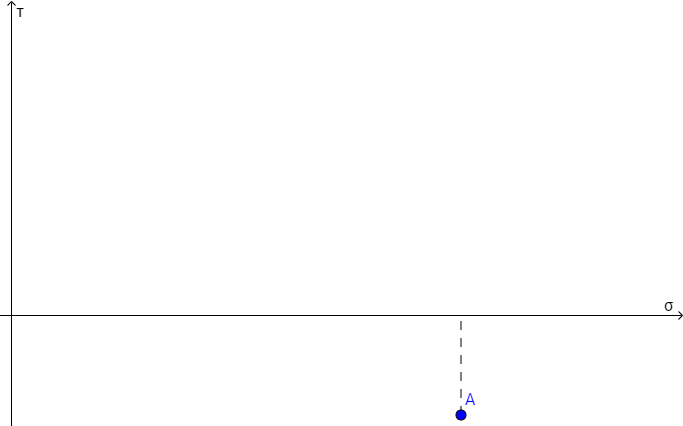
\includegraphics[width=0.5\linewidth,keepaspectratio]{mohr_a.png}
\end{center}

\item Marcar el punto $B=(\sigma_{y},\tau_{yx})$

\begin{center}
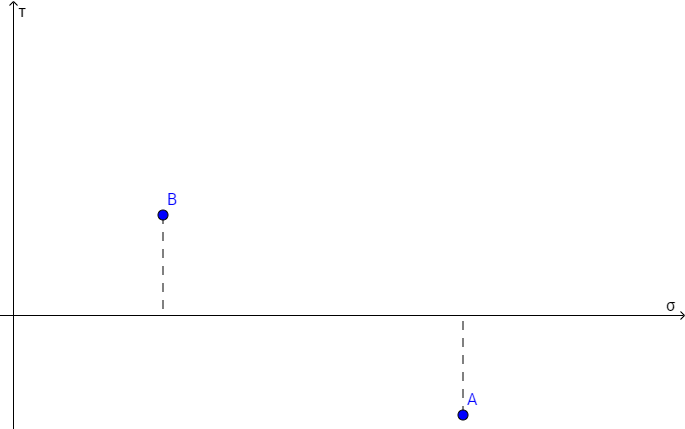
\includegraphics[width=0.5\linewidth,keepaspectratio]{mohr_b.png}
\end{center}

\item Unir $A$ y $B$:

\begin{center}
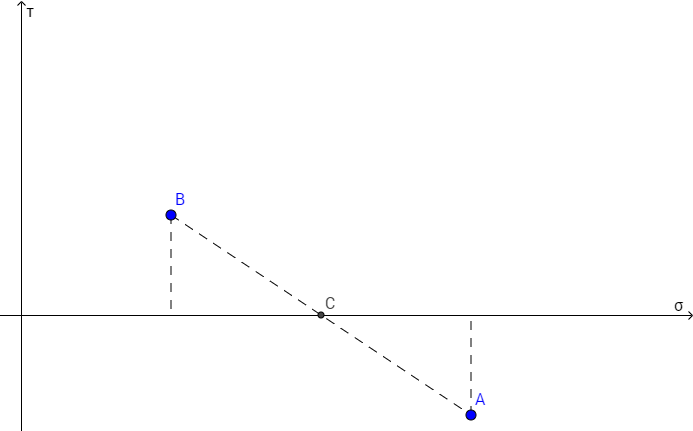
\includegraphics[width=0.5\linewidth,keepaspectratio]{mohr_ab.png}
\end{center}

\item El punto $C$ donde $\mathbf{AB}$ corta al eje $\sigma$ será el centro del círculo:

\begin{center}
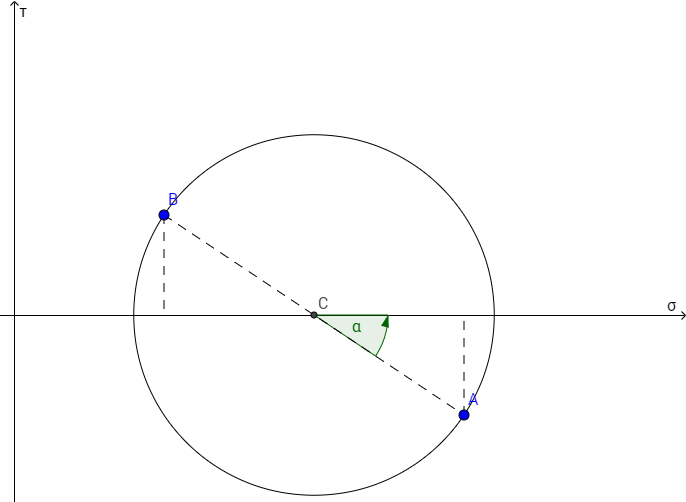
\includegraphics[width=0.5\linewidth,keepaspectratio]{mohr_circle.png}
\end{center} 
\end{enumerate}

En el círculo de Mohr, $\alpha=2\theta\implies\theta=\frac{\alpha}{2}$

\subsection*{Tensiones Principales}

Las \textbf{tensiones principales} son los autovalores de $\tau_{ij}$:

\[
|\tau_{ij}-\sigma\delta_{ij}|=
\left|\left(\begin{matrix}
\tau_{11} & \tau_{12} & \tau_{13} \\
\tau_{21} & \tau_{22} & \tau_{23} \\
\tau_{31} & \tau_{32} & \tau_{33} \\
\end{matrix}\right)-\sigma
\left(\begin{matrix}
1 & 0 & 0 \\
0 & 1 & 0 \\
0 & 0 & 1 \\
\end{matrix}\right)\right|=
\left|\begin{matrix}
\tau_{11}-\sigma & \tau_{13} & \tau_{13} \\
\tau_{21} & \tau_{22}-\sigma & \tau_{23} \\
\tau_{31} & \tau_{32} & \tau_{33}-\sigma \\
\end{matrix}\right|
\]

\[
=-\sigma^{3}+I_{1}\sigma^{2}-I_{2}\sigma+I_{3}=0
\]

$I_{1}$, $I_{2}$ y $I_{3}$ son invariantes y se calculan de la siguiente manera:

\begin{itemize}
\item \textit{Suma de los elementos de la diagonal: }$I_{1} = \tau_{11}+\tau_{22}+\tau_{33}$

\item \textit{Suma de los determinantes menores que se obtienen de recorrer la diagonal pero sin multiplicar por el pivote: }
\[
I_{2}=
\left|\begin{matrix}
\tau_{22} & \tau_{23} \\
\tau_{32} & \tau_{33} \\
\end{matrix}\right|
+
\left|\begin{matrix}
\tau_{11} & \tau_{13} \\
\tau_{31} & \tau_{33} \\
\end{matrix}\right|
+
\left|\begin{matrix}
\tau_{11} & \tau_{12} \\
\tau_{21} & \tau_{22} \\
\end{matrix}\right|
\]

\item \textit{Determinante de $\tau_{ij}$: }
\[
I_{3}=
\left|
\begin{matrix}
\tau_{11} & \tau_{13} & \tau_{13} \\
\tau_{21} & \tau_{22} & \tau_{23} \\
\tau_{31} & \tau_{32} & \tau_{33} \\
\end{matrix}
\right|
\]
\end{itemize}

Las \textbf{direcciones principales} son los autovectores de $\tau_{ij}$:

\[
(\tau_{ij}-\sigma\delta_{ij})\cdot\nu_{j}=
\left(\begin{matrix}
\tau_{11}-\sigma & \tau_{13} & \tau_{13} \\
\tau_{21} & \tau_{22}-\sigma & \tau_{23} \\
\tau_{31} & \tau_{32} & \tau_{33}-\sigma \\
\end{matrix}\right)\cdot
\left(\begin{matrix}
\stackrel \sigma \nu_{1} \\
\stackrel \sigma \nu_{2} \\
\stackrel \sigma \nu_{3} \\
\end{matrix}\right)=0
\]

Se puede conformar la matriz de rotación $\beta$ a partir de los autovectores:

\[
\beta=
\left(\begin{matrix}
\stackrel \sigma \nu_{1} & \stackrel \sigma \nu_{2} & \stackrel \sigma \nu_{3} \\
\stackrel \sigma \nu_{1} & \stackrel \sigma \nu_{2} & \stackrel \sigma \nu_{3} \\
\stackrel \sigma \nu_{1} & \stackrel \sigma \nu_{2} & \stackrel \sigma \nu_{3} \\
\end{matrix}\right);\quad
|\beta|>0
\]

Cada fila de $\beta$ es un autovector correspondiente a un determinado autovalor. La disposición correcta de las filas será aquella que haga que el determinante de la matriz sea mayor que cero (dextrógira).

\begin{thebibliography}{1}
\bibitem{MCF}
Y. C. Fung,
\emph{A First Course in Continuum Mechanics}, 
tercera edición,
PRENTICE HALL,
1994.
\end{thebibliography}

\end{document}